% Options for packages loaded elsewhere
\PassOptionsToPackage{unicode}{hyperref}
\PassOptionsToPackage{hyphens}{url}
%
\documentclass[
]{report}
\usepackage{lmodern}
\usepackage{setspace}
\usepackage{amssymb,amsmath}
\usepackage{ifxetex,ifluatex}
\ifnum 0\ifxetex 1\fi\ifluatex 1\fi=0 % if pdftex
  \usepackage[T1]{fontenc}
  \usepackage[utf8]{inputenc}
  \usepackage{textcomp} % provide euro and other symbols
\else % if luatex or xetex
  \usepackage{unicode-math}
  \defaultfontfeatures{Scale=MatchLowercase}
  \defaultfontfeatures[\rmfamily]{Ligatures=TeX,Scale=1}
\fi
% Use upquote if available, for straight quotes in verbatim environments
\IfFileExists{upquote.sty}{\usepackage{upquote}}{}
\IfFileExists{microtype.sty}{% use microtype if available
  \usepackage[]{microtype}
  \UseMicrotypeSet[protrusion]{basicmath} % disable protrusion for tt fonts
}{}
\makeatletter
\@ifundefined{KOMAClassName}{% if non-KOMA class
  \IfFileExists{parskip.sty}{%
    \usepackage{parskip}
  }{% else
    \setlength{\parindent}{0pt}
    \setlength{\parskip}{6pt plus 2pt minus 1pt}}
}{% if KOMA class
  \KOMAoptions{parskip=half}}
\makeatother
\usepackage{xcolor}
\IfFileExists{xurl.sty}{\usepackage{xurl}}{} % add URL line breaks if available
\IfFileExists{bookmark.sty}{\usepackage{bookmark}}{\usepackage{hyperref}}
\hypersetup{
  pdftitle={Contributions to Modern Bayesian Multilevel Modeling},
  pdfauthor={Alexander Knudson},
  hidelinks,
  pdfcreator={LaTeX via pandoc}}
\urlstyle{same} % disable monospaced font for URLs
\usepackage[top=1.0in,left=1.5in,bottom=1.25in,right=1.5in]{geometry}
\usepackage{color}
\usepackage{fancyvrb}
\newcommand{\VerbBar}{|}
\newcommand{\VERB}{\Verb[commandchars=\\\{\}]}
\DefineVerbatimEnvironment{Highlighting}{Verbatim}{commandchars=\\\{\}}
% Add ',fontsize=\small' for more characters per line
\usepackage{framed}
\definecolor{shadecolor}{RGB}{248,248,248}
\newenvironment{Shaded}{\begin{snugshade}}{\end{snugshade}}
\newcommand{\AlertTok}[1]{\textcolor[rgb]{0.94,0.16,0.16}{#1}}
\newcommand{\AnnotationTok}[1]{\textcolor[rgb]{0.56,0.35,0.01}{\textbf{\textit{#1}}}}
\newcommand{\AttributeTok}[1]{\textcolor[rgb]{0.77,0.63,0.00}{#1}}
\newcommand{\BaseNTok}[1]{\textcolor[rgb]{0.00,0.00,0.81}{#1}}
\newcommand{\BuiltInTok}[1]{#1}
\newcommand{\CharTok}[1]{\textcolor[rgb]{0.31,0.60,0.02}{#1}}
\newcommand{\CommentTok}[1]{\textcolor[rgb]{0.56,0.35,0.01}{\textit{#1}}}
\newcommand{\CommentVarTok}[1]{\textcolor[rgb]{0.56,0.35,0.01}{\textbf{\textit{#1}}}}
\newcommand{\ConstantTok}[1]{\textcolor[rgb]{0.00,0.00,0.00}{#1}}
\newcommand{\ControlFlowTok}[1]{\textcolor[rgb]{0.13,0.29,0.53}{\textbf{#1}}}
\newcommand{\DataTypeTok}[1]{\textcolor[rgb]{0.13,0.29,0.53}{#1}}
\newcommand{\DecValTok}[1]{\textcolor[rgb]{0.00,0.00,0.81}{#1}}
\newcommand{\DocumentationTok}[1]{\textcolor[rgb]{0.56,0.35,0.01}{\textbf{\textit{#1}}}}
\newcommand{\ErrorTok}[1]{\textcolor[rgb]{0.64,0.00,0.00}{\textbf{#1}}}
\newcommand{\ExtensionTok}[1]{#1}
\newcommand{\FloatTok}[1]{\textcolor[rgb]{0.00,0.00,0.81}{#1}}
\newcommand{\FunctionTok}[1]{\textcolor[rgb]{0.00,0.00,0.00}{#1}}
\newcommand{\ImportTok}[1]{#1}
\newcommand{\InformationTok}[1]{\textcolor[rgb]{0.56,0.35,0.01}{\textbf{\textit{#1}}}}
\newcommand{\KeywordTok}[1]{\textcolor[rgb]{0.13,0.29,0.53}{\textbf{#1}}}
\newcommand{\NormalTok}[1]{#1}
\newcommand{\OperatorTok}[1]{\textcolor[rgb]{0.81,0.36,0.00}{\textbf{#1}}}
\newcommand{\OtherTok}[1]{\textcolor[rgb]{0.56,0.35,0.01}{#1}}
\newcommand{\PreprocessorTok}[1]{\textcolor[rgb]{0.56,0.35,0.01}{\textit{#1}}}
\newcommand{\RegionMarkerTok}[1]{#1}
\newcommand{\SpecialCharTok}[1]{\textcolor[rgb]{0.00,0.00,0.00}{#1}}
\newcommand{\SpecialStringTok}[1]{\textcolor[rgb]{0.31,0.60,0.02}{#1}}
\newcommand{\StringTok}[1]{\textcolor[rgb]{0.31,0.60,0.02}{#1}}
\newcommand{\VariableTok}[1]{\textcolor[rgb]{0.00,0.00,0.00}{#1}}
\newcommand{\VerbatimStringTok}[1]{\textcolor[rgb]{0.31,0.60,0.02}{#1}}
\newcommand{\WarningTok}[1]{\textcolor[rgb]{0.56,0.35,0.01}{\textbf{\textit{#1}}}}
\usepackage{longtable,booktabs}
% Correct order of tables after \paragraph or \subparagraph
\usepackage{etoolbox}
\makeatletter
\patchcmd\longtable{\par}{\if@noskipsec\mbox{}\fi\par}{}{}
\makeatother
% Allow footnotes in longtable head/foot
\IfFileExists{footnotehyper.sty}{\usepackage{footnotehyper}}{\usepackage{footnote}}
\makesavenoteenv{longtable}
\usepackage{graphicx,grffile}
\makeatletter
\def\maxwidth{\ifdim\Gin@nat@width>\linewidth\linewidth\else\Gin@nat@width\fi}
\def\maxheight{\ifdim\Gin@nat@height>\textheight\textheight\else\Gin@nat@height\fi}
\makeatother
% Scale images if necessary, so that they will not overflow the page
% margins by default, and it is still possible to overwrite the defaults
% using explicit options in \includegraphics[width, height, ...]{}
\setkeys{Gin}{width=\maxwidth,height=\maxheight,keepaspectratio}
% Set default figure placement to htbp
\makeatletter
\def\fps@figure{htbp}
\makeatother
\setlength{\emergencystretch}{3em} % prevent overfull lines
\providecommand{\tightlist}{%
  \setlength{\itemsep}{0pt}\setlength{\parskip}{0pt}}
\setcounter{secnumdepth}{5}
\usepackage[]{natbib}
\bibliographystyle{apalike}

\title{Contributions to Modern Bayesian Multilevel Modeling}
\author{Alexander Knudson}
\date{Monday August 03, 2020}

\begin{document}
\maketitle

{
\setcounter{tocdepth}{2}
\tableofcontents
}
\listoftables
\listoffigures
\setstretch{2}
\hypertarget{abstract}{%
\chapter*{Abstract}\label{abstract}}


\textbf{Big Idea:} \emph{making contributions to \& gaining mastery of state of the art statistical computing tools and Bayesian modeling/probabilistic programming.}

\hypertarget{acknowledgments}{%
\chapter*{Acknowledgments}\label{acknowledgments}}


I would like to first and foremost thank my sister Heather for always being a constant source of sarcasm and teasing. Without her skepticism I would not have had enough motivation to finish this degree out of spite, and instead would have had to rely on self-discipline and encouragement from my peers and mentors.

\hypertarget{introduction}{%
\chapter{Introduction}\label{introduction}}

\begin{itemize}
\tightlist
\item
  Soft intro to modern computing, analysis

  \begin{itemize}
  \tightlist
  \item
    advance in CPU+programming leads to evolved statistical methods

    \begin{itemize}
    \tightlist
    \item
      ML/DL, high dimensional analysis, big data, Bayesian techniques
    \end{itemize}
  \item
    multidisciplinary techniques; numerical methods, probability theory, statistics, computer science, visualizations, etc

    \begin{itemize}
    \tightlist
    \item
      root finding, change of variables, Gaussian quadrature, Hermite polynomials, Monte Carlo simulation, floating point arithmetic
    \end{itemize}
  \item
    Organization and reproducibility are crucial in a data analysis setting

    \begin{itemize}
    \tightlist
    \item
      pre-planning, modularity, workflows, versioning, virtual environments, DRY programming, code that is easy to read
    \end{itemize}
  \item
    Clean data is important for good modeling

    \begin{itemize}
    \tightlist
    \item
      garbage in leads to garbage out
    \end{itemize}
  \end{itemize}
\end{itemize}

With the advances in computational power and high-level programming languages like Python, R, and Julia, statistical methods have evolved to be more flexible and expressive.

\begin{itemize}
\tightlist
\item
  Overview of classical modeling methods

  \begin{itemize}
  \tightlist
  \item
    classical approaches to data analysis usually adhere to the flexibility-interpretability trade-off
  \item
    generally inflexible (parametric) to be more interpretable and computationally easier
  \item
    sometimes a model is too flexible (non-parametric) and loses crucial inferential power
  \item
    sometimes our assumptions about the data are invalid

    \begin{itemize}
    \tightlist
    \item
      normality, independence, heteroskedacity, etc.
    \end{itemize}
  \item
    often limited when it comes to statistical summaries and confidence intervals
  \end{itemize}
\item
  Solutions or alternatives when classical models fail

  \begin{itemize}
  \tightlist
  \item
    Bayesian inference is a powerful, descriptive, and flexible modeling framework
  \item
    Bayes theorem is a simple model of incorporating prior information and data to produce a posterior probability or distribution
  \item
    \(P(\theta | X) \propto P(X | \theta) * P(\theta)\) or \(posterior \propto prior \times likelihood\)

    \begin{itemize}
    \tightlist
    \item
      The prior is some distribution over the parameter space
    \item
      The likelihood is the probability of an outcome in the sample space given a value in the parameter space
    \item
      The posterior is the likelihood of values in the parameter space after observing values from the sample space
    \end{itemize}
  \item
    Bayesian statistics, when described without math, actually feels natural to most people

    \begin{itemize}
    \tightlist
    \item
      you hear hoof beats, you think horses, not zebras {[}unless you're in Africa, but that's prior information ;){]}
    \end{itemize}
  \item
    The catch is that the model is not complete as written above
  \item
    There is actually a denominator in Bayes' Theorem

    \begin{itemize}
    \tightlist
    \item
      \(P(\theta | X) = \frac{P(X | \theta)\cdot P(\theta)}{\sum_i P(X | \theta_i)} = \frac{P(X | \theta)\cdot P(\theta)}{\int_\Omega P(X | \theta)d\theta}\)
    \item
      In general, the denominator is not known, or is not not easy (or possible) to calculate, but it always evaluates to a constant (hence the ``proportional to'')
    \item
      The denominator acts as a scaling value that forces \(P(\theta|X)\) to be a probability distribution (i.e.~area under PDF is equal to 1)
    \item
      There are simulation-based techniques that let one approximate the posterior distribution without needing to know the analytic solution to the denominator
    \end{itemize}
  \end{itemize}
\end{itemize}

I have organized this thesis as follows. In \protect\hyperlink{motivating-data}{Chapter 2} I introduce the data set that drives the narrative and that motivates the adoption of Bayesian multilevel modeling. In \protect\hyperlink{background}{Chapter 3} there is a review of common approaches approaches to modeling with psychometric data, and the benefits and drawbacks of such techniques. \protect\hyperlink{bayesian-modeling}{Chapter 4} introduces Bayesian hierarchical modeling and programming frameworks for Bayesian inference. In \protect\hyperlink{workflow}{Chapter 5} I describe and work through a principled Bayesian workflow for multilevel modeling. \protect\hyperlink{model-checking}{Chapter 6} goes into more depth on checking the model goodness of fit and model diagnostics in a Bayesian setting. Finally in \protect\hyperlink{predictive-inference}{Chapter 7} I demonstrate how to use the Bayesian model from the principled workflow for predictive inference, and use posterior predictive distributions to plot and compare models.

\hypertarget{motivating-data}{%
\chapter{Background and Motivating Data}\label{motivating-data}}

It was Charles Darwin who in his book \emph{On the Origin of Species} developed the idea that living organisms adapt to better survive in their environment. Sir Francis Galton, inspired by Darwin's ideas, became interested in the differences in human beings and in how to measure those differences. Though the dark side of statistics and hubris lead Galton to become a pioneer of eugenics, his works on studying and measuring human differences lead to the creation of psychometrics -- the science of measuring mental faculties. Around the same time that was developing his theories, Johann Friedrich Herbart was also interested in studying consciousness through the scientific method, and is responsible for creating mathematical models of the mind.

E.H. Weber built upon Herbart's work, and sought out to prove the idea of a psychological threshold. A psychological threshold is a minimum stimulus intensity necessary to activate a sensory system -- a \emph{liminal} stimulus. He paved the way for experimental psychology and is the namesake of \emph{Weber's Law} -- the change in a stimulus that will be just noticeable is a constant ratio of the original stimulus \citep{britannica2014editors}.

\[
\frac{\Delta I}{I} = k
\]

To put this law into practice, consider holding a 1 kg weight (\(I = 1\)), and further suppose that we can \emph{just} detect the difference between a 1 kg weight and a 1.2 kg weight (\(\Delta I = 0.2\)). Then the constant just noticeable ratio is

\[
k = \frac{0.2}{1} = 0.2
\]

So now if we pick up a 10 kg weight, we should be able to determine how much more mass is required to just detect a difference:

\[
\frac{\Delta I}{10} = 0.2 \Rightarrow \Delta I = 2
\]

The difference between a 10 kg and a 12 kg weight should be just barely perceptible. Notice that the difference in the first set of weights is 0.2 and in the second set it is 2. Our perception of the difference in stimulus intensities is not absolute, but relative. G.T. Fechner devised the law (Weber-Fechner Law) that the strength of a sensation grows as the logarithm of the stimulus intensity.

\[S = K \ln I\]

An example to this law is to consider two light sources, one that is 100 lumens (\(S_1 = K \ln 100\)) and another that is 200 lumens (\(S_2 = K \ln 200\)). The intensity of the second light is not perceived as twice as bright, but only about 1.15 times as bright according to the Weber-Fechner law: \(\theta = S_2 / S_1 \approx 1.15\). Notice that the value \(K\) cancels out when calculating the relative intensity, but knowing \(K\) can lead to important psychological insights; insights about differences between persons or groups of people! What biological and contextual factors affect how people perceive different stimuli? How do we measure their perception in a meaningful way? As one might expect, we can collect data from psychometric experiments, fit a model to the data from a family of functions called \emph{psychometric functions}, and inspect key operating characteristics of those functions.

\hypertarget{psychometric-experiments}{%
\section{Psychometric Experiments}\label{psychometric-experiments}}

Psychometric experiments are devised in a way to examine psychophysical processes, or the response between the world around us and our inward perceptions. A \textbf{psychometric function} relates an observer's performance to an independent variable, usually some physical quantity of a stimulus in a psychophysical task \citep{wichmann2001a}. Psychometric functions were studied as early as the late 1800's, and Edwin Boring published a chart of the psychometric function in The American Journal of Psychology in 1917 \citep{boring1917chart}.

\begin{figure}

{\centering 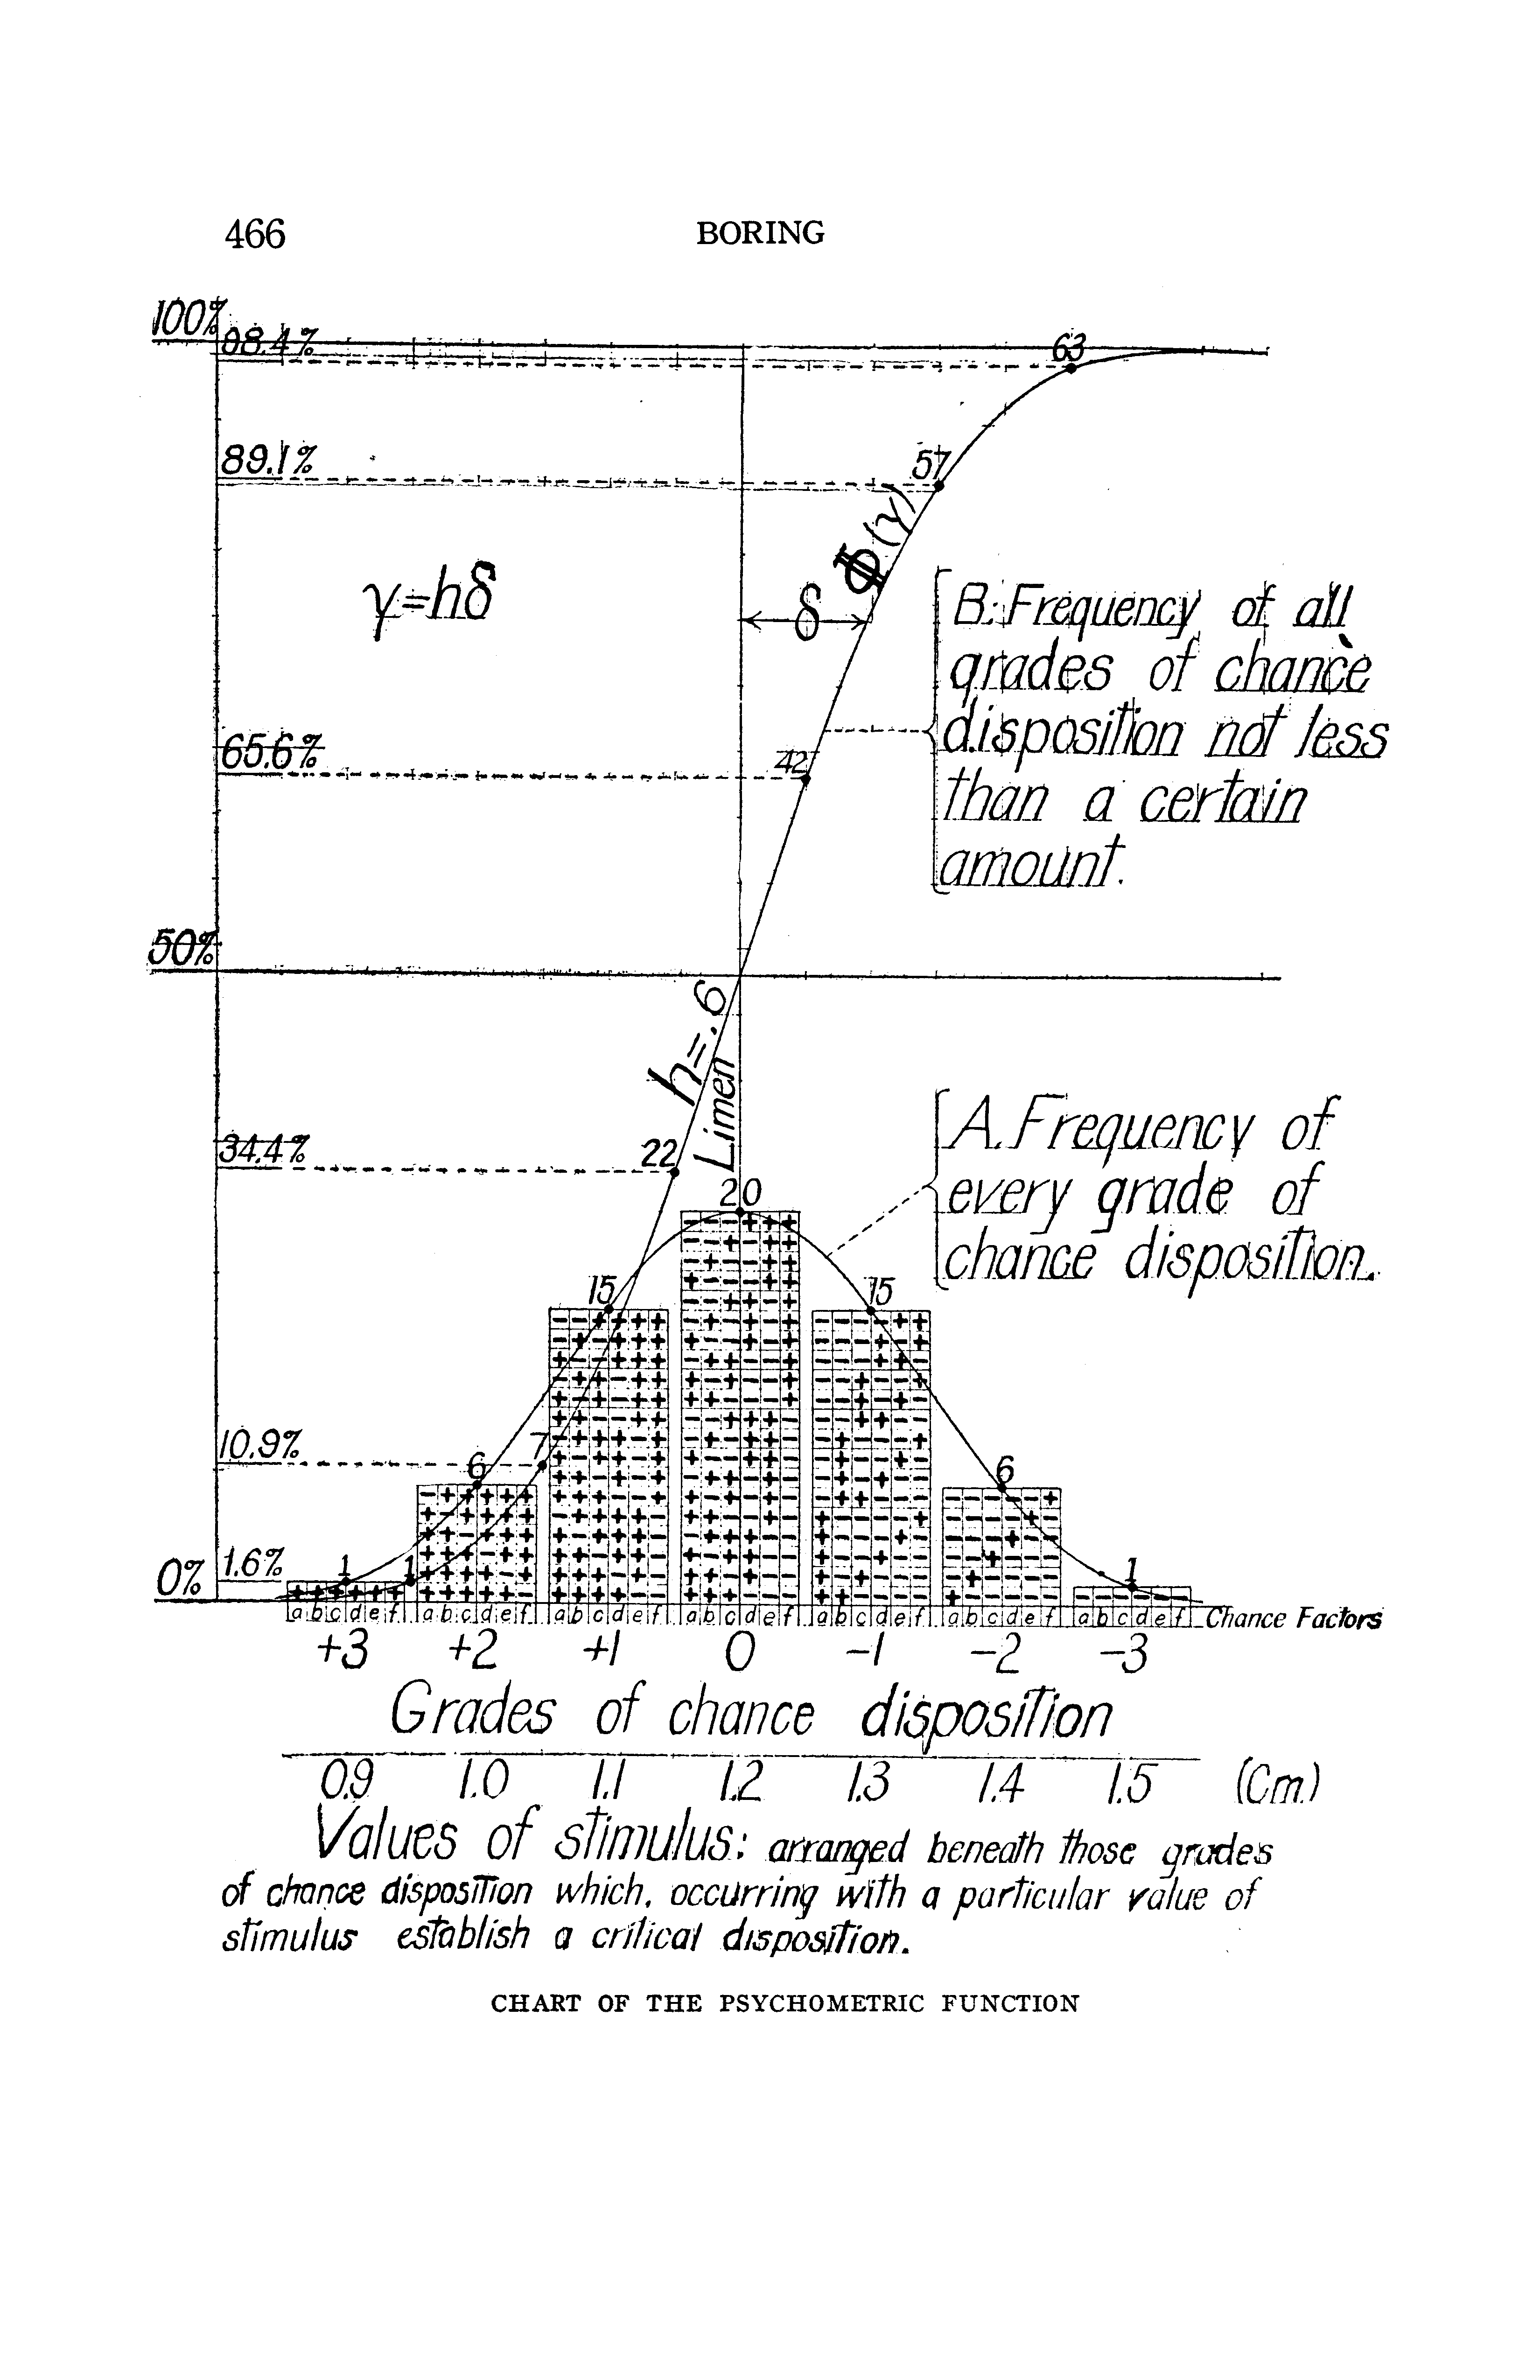
\includegraphics[width=0.7\linewidth]{figures/chart_of_pf} 

}

\caption{A chart of the psychometric function. The experiment in this paper places two points on a subject's skin separated by some distance, and has them answer their impression of whether there is one point or 'two', recorded as either 'two' or 'not two'. As the separation of aesthesiometer points increases, so too does the subject's confidence in their response of 'two'. So at what separation is the impression of two points liminal?}\label{fig:chart-of-pf}
\end{figure}

Figure \ref{fig:chart-of-pf} displays the key aspects of the psychometric function. The most crucial part is the sigmoid function, the S-like non-decreasing curve, which in this case is represented by the Normal CDF, \(\Phi(\gamma)\). The horizontal axis represents the stimulus stimulus intensity, the separation of two points in centimeters. The vertical axis represents the probability that a subject has the impression of two points. With only experimental data, the response proportion becomes an approximation for the probability.

This leads me to talk about the type of psychometric experiment that this paper deals with called a \textbf{temporal order judgment} (TOJ) experiment. The concept is that if there are two distinct stimuli occurring nearly simultaneously then our brains will bind them into a single percept -- perceive them as happening simultaneously. Compensation for small temporal differences is beneficial for coherent multisensory experiences, particularly in visual-speech synthesis as it is necessary to maintain an accurate representation of the sources of multisensory events. The temporal asynchrony between stimuli is called the \textbf{stimulus onset asynchrony} (SOA), and the range of SOAs for which sensory signals are integrated into a global percept is called the \textbf{temporal binding window}. When the SOA grows too large then the brain segregates the two signals and the temporal order can be determined.

Our experiences in life as we age shape the mechanisms of processing multisensory signals, and some multisensory signals are integrated much more readily than others. Perceptual synchrony has been previously studied through the \textbf{point of subjective simultaneity} (PSS) -- the temporal delay between two signals at which an observer is unsure about their temporal order \citep{stone2001now}. The temporal binding window is the time span over which sensory signals arising from different modalities appear integrated into a global percept. A deficit in temporal sensitivity may lead to a widening of the temporal binding window and reduce the ability to segregate unrelated sensory signals. In temporal order judgment tasks, the ability to discriminate the timing of multiple sensory signals is referred to as temporal sensitivity, and is studied through the measurement of the \textbf{just noticeable difference} (JND) -- the smallest lapse in time so that a temporal order can just be determined. Figure \ref{fig:plot-ref-pf} highlights the features through which we study psychometric functions. The PSS is defined as the point where an observer can do no better at determining temporal order than random guessing (i.e.~the response probability is 50\%). The JND is defined as the extra temporal delay between stimuli so that the temporal order is just able to be determined. Historically this has been defined as the difference between the 84\% level and the PSS, though the upper level depends on domain expertise.

\begin{figure}

{\centering 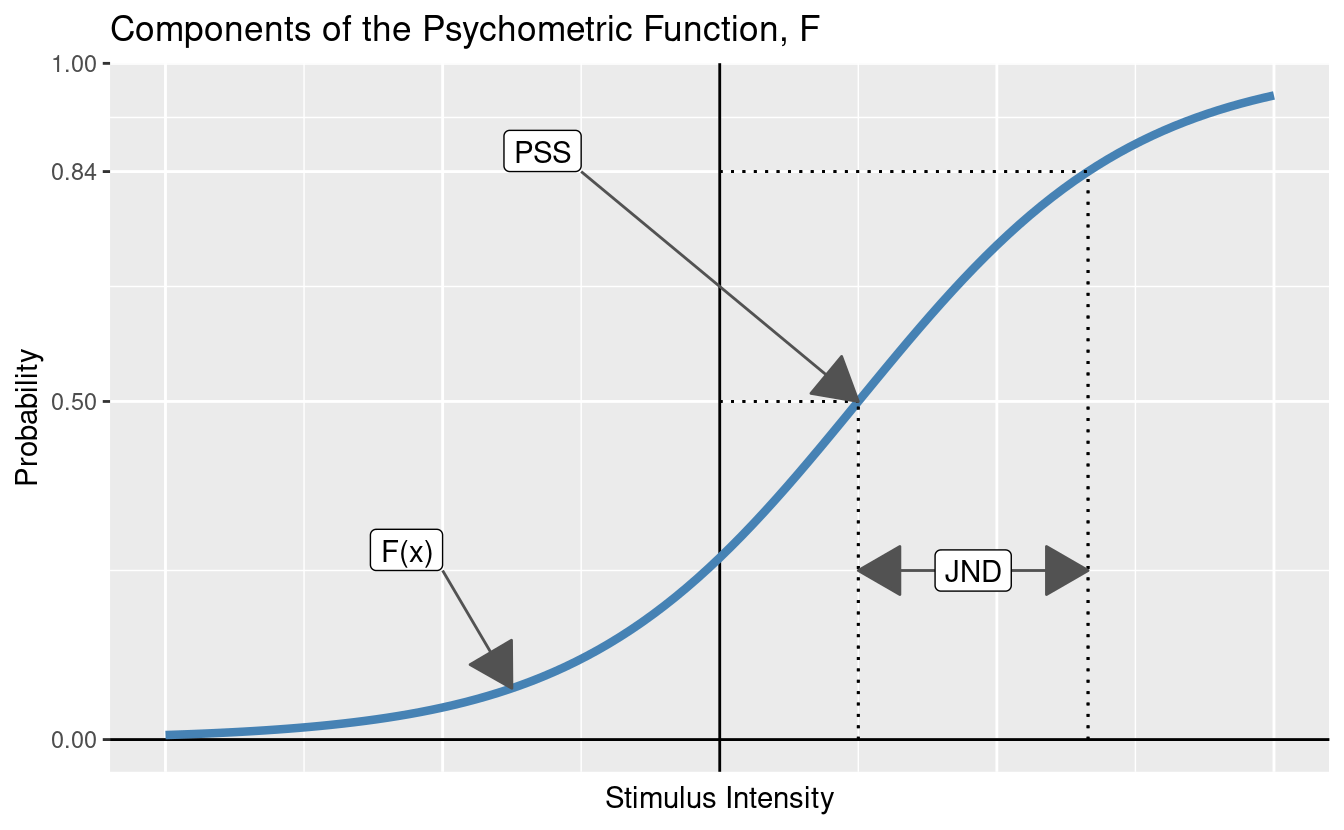
\includegraphics[width=0.7\linewidth]{adknudson-thesis_files/figure-latex/plot-ref-pf-1} 

}

\caption{The PSS is defined as the point where an observer can do no better at determining temporal order than random guessing. The just noticeable difference is defined as the extra temporal delay between stimuli so that the temporal order is just able to be determined. Historically this has been defined as the difference between the 0.84 level and the PSS, though the upper level depends on domain expertise.}\label{fig:plot-ref-pf}
\end{figure}

Perceptual synchrony and temporal sensitivity can be modified through a baseline understanding. In order to perceive physical events as simultaneous, our brains must adjust for differences in temporal delays of transmission of both psychical signals and sensory processing \citep{fujisaki2004recalibration}. In some cases such as with audiovisual stimuli, the perception of simultaneity can be modified by repeatedly presenting the audiovisual stimuli at fixed time separations (called an adapter stimulus) to an observer \citep{vroomen2004recalibration}. This repetition of presenting the adapter stimulus is called \textbf{temporal recalibration}.

The data set that I introduce in the next section concerns temporal order judgment across various sensory modalities with a temporal recalibration component.

\hypertarget{temporal-order-judgment-data}{%
\section{Temporal Order Judgment Data}\label{temporal-order-judgment-data}}

The data set that I am using in this paper comes from experiments done by A.N. Scurry and Dr.~Fang Jiang in the Department of Psychology at the University of Nevada. Reduced temporal sensitivity in the aging population manifests in an impaired ability to perceive synchronous events as simultaneous, and similarly more difficulty in segregating asynchronous sensory signals that belong to different sources. The consequences of a widening of the temporal binding window is considered in \citet{scurry2019aging}, as well as a complete detailing of the experimental setup and recording process. I provide a shortened summary of the methods.

There are four different tasks in the experiment: audio-visual, visual-visual, visuo-motor, and duration, and I will refer to each task respectively as audiovisual, visual, sensorimotor, and duration. The participants consist of 15 young adults (age 20-27), 15 middle age adults (age 39-50), and 15 older adults (age 65-75), all recruited from the University of Nevada, Reno. Additionally all subjects are right handed and were reported to have normal or corrected to normal hearing and vision.

\begin{table}[!h]

\caption{\label{tab:multitask-data}Sample of motivating data}
\centering
\begin{tabular}[t]{rrlllllrl}
\toprule
soa & response & rid & sid & task & trial & age\_group & age & sex\\
\midrule
350 & 1 & av-post2-O-f-BB & O-f-BB & audiovisual & post2 & older\_adult & 68 & F\\
0 & 0 & dur-post1-M-m-WW & M-m-WW & duration & post1 & middle\_age & 50 & M\\
-1 & 1 & sm-pre-O-f-MW & O-f-MW & sensorimotor & pre & older\_adult & 69 & F\\
-225 & 0 & vis-pre-M-f-CC & M-f-CC & visual & pre & middle\_age & 39 & F\\
\bottomrule
\end{tabular}
\end{table}

\hypertarget{background}{%
\chapter{Background to Modeling}\label{background}}

\begin{itemize}
\tightlist
\item
  Generalized Linear Models

  \begin{itemize}
  \tightlist
  \item
    classical approaches to fitting/estimation

    \begin{itemize}
    \tightlist
    \item
      Maximum likelihood estimation

      \begin{itemize}
      \tightlist
      \item
        Simple and almost every piece of statistical software will have an implementation
      \end{itemize}
    \end{itemize}
  \item
    Expectation Maximization
  \item
    Random effects (Gelmen and Hill)
  \item
    Bayesian GLMs

    \begin{itemize}
    \tightlist
    \item
      Completely reliant on MCMC
    \end{itemize}
  \end{itemize}
\item
  Model-free estimations (footnote? remark?)

  \begin{itemize}
  \tightlist
  \item
    non-parametric models
  \item
    \citep{zchaluk2009model}
  \end{itemize}
\item
  Bayesian logistic regression

  \begin{itemize}
  \tightlist
  \item
    \citet{gelman2008weakly}
  \item
    Can't completely express the structure (hierarchy) of the data
  \end{itemize}
\item
  Residual Analysis

  \begin{itemize}
  \item
    using the fitted values vs.~the observed values to evaluate goodness of fit
  \item
  \end{itemize}
\item
  So what's the answer?

  \begin{itemize}
  \tightlist
  \item
    The last two options (bayes + multilevel) when on their own do well, but are not robust to
  \end{itemize}
\item
  shortcomings

  \begin{itemize}
  \item
    Convergence failure in the presence of complete separation

    \begin{itemize}
    \tightlist
    \item
      \citep{prins2019too}, \citep{ghosh2018use}
    \end{itemize}
  \item
  \end{itemize}
\end{itemize}

\hypertarget{bayesian-modeling}{%
\chapter{Bayesian Multilevel Modeling}\label{bayesian-modeling}}

\begin{itemize}
\tightlist
\item
  short intro

  \begin{itemize}
  \tightlist
  \item
    sentence 1
  \item
    sentence 2
  \item
    sentence 3
  \end{itemize}
\end{itemize}

\hypertarget{bayesian-stuff}{%
\section{Bayesian Stuff}\label{bayesian-stuff}}

\begin{itemize}
\item
  Mathematical foundations

  \begin{itemize}
  \tightlist
  \item
    Bayes rule in regression setting
  \end{itemize}
\item
  Easy in theory, difficult in practice

  \begin{itemize}
  \tightlist
  \item
    Example of a conjugate priors
  \item
    need more complexity -\textgreater{} computer methods
  \item
    Computer methods needed
  \end{itemize}
\item
\end{itemize}

\hypertarget{multilevel-modeling-stuff}{%
\section{Multilevel Modeling Stuff}\label{multilevel-modeling-stuff}}

\begin{itemize}
\item
  Estimating the variance at different levels in the model
\item
\end{itemize}

\hypertarget{workflow}{%
\chapter{Principaled Bayesian Workflow}\label{workflow}}

\begin{itemize}
\tightlist
\item
  Standardizing Predictors
\item
  Parameterization of the linear predictor

  \begin{itemize}
  \tightlist
  \item
    Choice of Link Function
  \item
    Choice of Priors
  \item
    lapse rates
  \end{itemize}
\end{itemize}

\hypertarget{feature-engineering}{%
\section{Feature Engineering}\label{feature-engineering}}

\hypertarget{prior-specification}{%
\section{Prior Specification}\label{prior-specification}}

\hypertarget{model-checking}{%
\chapter{Model Checking}\label{model-checking}}

\begin{itemize}
\tightlist
\item
  The problem of simulating multivariate data with arbitrary marginal distributions
\item
  Copula approach

  \begin{itemize}
  \tightlist
  \item
    Nonlinear transformation that invalidates the correlation structure
  \end{itemize}
\item
  Kendall and Spearman matching

  \begin{itemize}
  \tightlist
  \item
    Nearest Positive Semidefinite correlation matrix

    \begin{itemize}
    \tightlist
    \item
      Semidefinte Programming (ProxSDP.jl)
    \item
      \url{https://arxiv.org/abs/1810.05231}
    \item
      Qi and Sun 2006 (quadratically convergent method)
    \end{itemize}
  \end{itemize}
\item
  Pearson matching

  \begin{itemize}
  \tightlist
  \item
    Chen 2001 (NORTARA)
  \item
    Xiao, Zhou 2019 (Numeric Approximation)
  \end{itemize}
\item
  Using synthetic data to design experiments

  \begin{itemize}
  \tightlist
  \item
    Bayesian p-value
  \item
    How much data to notice an effect
  \item
    Bayesian hypothesis testing via predictive performance
  \end{itemize}
\end{itemize}

\hypertarget{predictive-inference}{%
\chapter{Predictive Inference}\label{predictive-inference}}

\begin{itemize}
\tightlist
\item
  Compare to conjugate model
\item
  Prior predictive distributions
\item
  Posterior predictive distributions
\item
  Calibrating the model
\item
  Use of synthetic data to assess model properties
\end{itemize}

\hypertarget{results}{%
\chapter{Results}\label{results}}

Objective conclusions

\hypertarget{discussion}{%
\chapter{Discussion}\label{discussion}}

Subjective conclusions

\hypertarget{conclusion}{%
\chapter{Conclusion}\label{conclusion}}

Really just placeholder stuff for now.

\[
\frac{1}{\sqrt{2\pi\sigma}} \exp{\left\lbrace \frac{(x-\mu)^2}{\sigma^2} \right\rbrace}
\]

\hypertarget{appendix-appendix}{%
\appendix \addcontentsline{toc}{chapter}{\appendixname}}


\hypertarget{supplementary-code}{%
\chapter{Supplementary Code}\label{supplementary-code}}

One model, Three Implementations. There are a few ways to specify a hierarchical model in R. Below I describe three common frameworks that require varying levels of mathematical and programmatic competence. Frameworks with lower barriers for entry are great for researchers in many fields, but they lack fine control over the parameters in a model. As the framework complexity increases, so too does the ability to generate complex models that are typically not possible.

Novice
\setstretch{1.0}

\begin{Shaded}
\begin{Highlighting}[]
\KeywordTok{library}\NormalTok{(rstanarm)}
\KeywordTok{stan_glmer}\NormalTok{(}\KeywordTok{cbind}\NormalTok{(k, n}\OperatorTok{-}\NormalTok{k) }\OperatorTok{~}\StringTok{ }\DecValTok{1} \OperatorTok{+}\StringTok{ }\NormalTok{x }\OperatorTok{+}\StringTok{ }\NormalTok{(}\DecValTok{1} \OperatorTok{+}\StringTok{ }\NormalTok{x }\OperatorTok{|}\StringTok{ }\NormalTok{G1) }\OperatorTok{+}\StringTok{ }\NormalTok{(}\DecValTok{1} \OperatorTok{+}\StringTok{ }\NormalTok{x }\OperatorTok{|}\StringTok{ }\NormalTok{G2), }
           \DataTypeTok{family =} \KeywordTok{binomial}\NormalTok{(}\DataTypeTok{link =} \StringTok{"logit"}\NormalTok{),}
           \DataTypeTok{data =}\NormalTok{ dat)}
\end{Highlighting}
\end{Shaded}

\setstretch{2.0}

Intermediate

\setstretch{1.0}

\begin{Shaded}
\begin{Highlighting}[]
\KeywordTok{library}\NormalTok{(rethinking)}
\KeywordTok{ulam}\NormalTok{(}\KeywordTok{alist}\NormalTok{(}
\NormalTok{  k }\OperatorTok{~}\StringTok{ }\KeywordTok{binomial}\NormalTok{(n, pi)}
  \KeywordTok{logit}\NormalTok{(pi) <-}\StringTok{ }\NormalTok{(a }\OperatorTok{+}\StringTok{ }\NormalTok{aG1[G1] }\OperatorTok{+}\StringTok{ }\NormalTok{aG2[G2]) }\OperatorTok{+}\StringTok{ }\NormalTok{(b }\OperatorTok{+}\StringTok{ }\NormalTok{bG1[G1] }\OperatorTok{+}\StringTok{ }\NormalTok{bG2[G2]) }\OperatorTok{*}\StringTok{ }\NormalTok{x,}
  
\NormalTok{  a }\OperatorTok{~}\StringTok{ }\KeywordTok{normal}\NormalTok{(}\DecValTok{0}\NormalTok{, }\DecValTok{10}\NormalTok{),}
\NormalTok{  aG1[G1] }\OperatorTok{~}\StringTok{ }\KeywordTok{normal}\NormalTok{(}\DecValTok{0}\NormalTok{, sd_aG1),}
\NormalTok{  aG2[G2] }\OperatorTok{~}\StringTok{ }\KeywordTok{normal}\NormalTok{(}\DecValTok{0}\NormalTok{, sd_aG2),}
  \KeywordTok{c}\NormalTok{(sd_aG1, sd_aG2) }\OperatorTok{~}\StringTok{ }\KeywordTok{half_cauchy}\NormalTok{(}\DecValTok{0}\NormalTok{, }\DecValTok{10}\NormalTok{),}

\NormalTok{  b }\OperatorTok{~}\StringTok{ }\KeywordTok{normal}\NormalTok{(}\DecValTok{0}\NormalTok{, }\DecValTok{10}\NormalTok{),}
\NormalTok{  bG1[G1] }\OperatorTok{~}\StringTok{ }\KeywordTok{normal}\NormalTok{(}\DecValTok{0}\NormalTok{, sd_bG1),}
\NormalTok{  bG2[G2] }\OperatorTok{~}\StringTok{ }\KeywordTok{normal}\NormalTok{(}\DecValTok{0}\NormalTok{, sd_bG2),}
  \KeywordTok{c}\NormalTok{(sd_bG1, sd_bG2) }\OperatorTok{~}\StringTok{ }\KeywordTok{half_cauchy}\NormalTok{(}\DecValTok{0}\NormalTok{, }\DecValTok{10}\NormalTok{)}
\NormalTok{), }\DataTypeTok{data =}\NormalTok{ dat, }\DataTypeTok{log_lik =} \OtherTok{TRUE}\NormalTok{)}
\end{Highlighting}
\end{Shaded}

\setstretch{2.0}

Advanced

\setstretch{1.0}

\begin{verbatim}
data{
    int<lower=0> N;
    int<lower=0> N_G1;
    int<lower=0> N_G2;
    int n[N];
    int k[N];
    int G1[N];
    int G2[N];
    int trt[N];
    vector[N] x;
}
parameters{
    real a;
    vector[N_G1] aG1;
    vector[N_G2] aG2;
    real b;
    vector[N_G1] bG1;
    vector[N_G2] bG2;
    real<lower=0> sd_aG1;
    real<lower=0> sd_aG2;
    real<lower=0> sd_bG1;
    real<lower=0> sd_bG2;
}
model{
    vector[N] p;
    a   ~ normal(0, 10);
    aG1 ~ normal(0, sd_aG1);
    aG2 ~ normal(0, sd_aG2);
    b   ~ normal(0, 10);
    bG1 ~ normal(0, sd_bG1);
    bG2 ~ normal(0, sd_bG2);
    sd_aG1 ~ cauchy(0, 10);
    sd_aG2 ~ cauchy(0, 10);
    sd_bG1 ~ cauchy(0, 10);
    sd_bG2 ~ cauchy(0, 10);
    for ( i in 1:N ) {
        p[i] = (a + aG1[G1[i]] + aG2[G2[i]]) + (b + bG1[G1[i]] + bG2[G2[i]]) * x[i];
    }
    k ~ binomial_logit(n , p);
}
\end{verbatim}

\setstretch{2.0}

\setstretch{1.0}

  \bibliography{bibliography.bib}

\end{document}
